\documentclass {article}

\usepackage{framed}
\usepackage{amsmath}
\usepackage{amssymb}
\usepackage{graphicx}
\usepackage{float}

\title{Assignment 3 for CS224d}
\author{Lifu Huang}
\date{April 2016}

\begin{document}
\maketitle
\section{RNN's(Recursive Neural Network)}
\subsection*{(a)}
\begin{align*}
\delta^{(s)} &= \hat{y} - y \\
\delta^{(1)} &= f'(h^{(1)}) \circ (U^T \delta^{(s)} + \delta_{above}) \\
\delta_{below} &= (W^{(1)})^T \delta^{(1)}
\\
\nabla_U J &= \delta^{(s)} (h^{(1)})^T \\
\nabla_{b^{(s)}} J &= \delta^{(s)} \\
\nabla_{W^{(1)}} J &= \delta^{(1)} \left[h^{(1)}_{left}; h^{(1)}_{right}\right]^T \\
\nabla_{b^{(1)}} J &= \delta^{(1)} \\
\nabla_{\left[L_{left};L_{right} \right]} J &= \delta_{below} \\
\end{align*}
\subsection*{(b)}
Please see code files for details.
\subsection*{(c)}
\subsubsection*{(a)}
\begin{figure}[H]
\centering
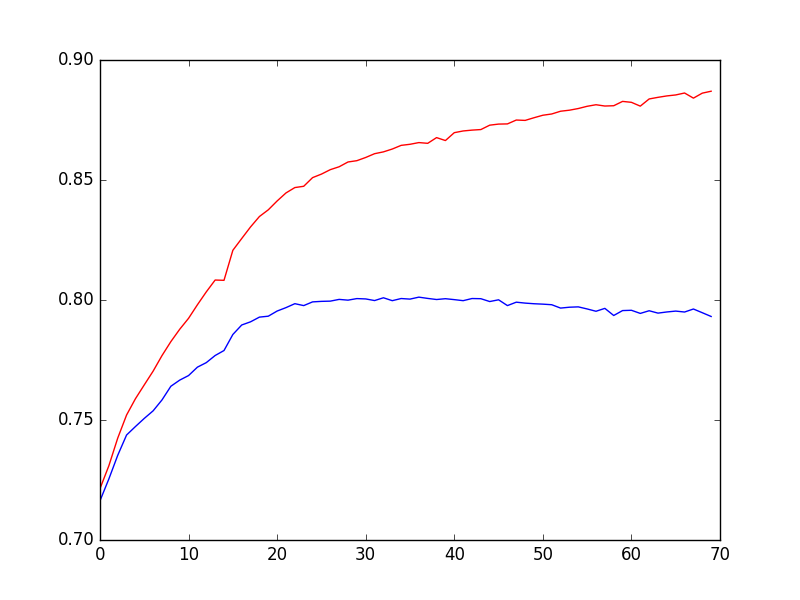
\includegraphics[width=0.7\linewidth]{ps3_1_c_a}
\caption{Accuracy on Training and Dev Set over Epochs}
\label{fig:ps3_1_c_a}
\end{figure}
\subsubsection*{(b)}
Beacause training for too many epochs may lead to the problem of over fitting.
\subsubsection*{(c)}
\begin{figure}[H]
\centering
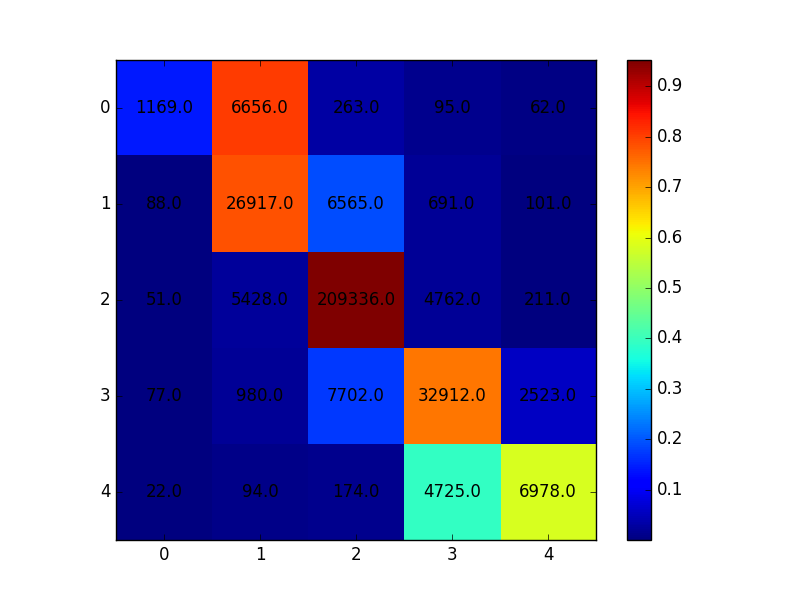
\includegraphics[width=0.7\linewidth]{ps3_1_c_c_train}
\caption{Confusion Matrix on Training Set}
\label{fig:ps3_1_c_c_train}
\end{figure}
\begin{figure}[H]
\centering
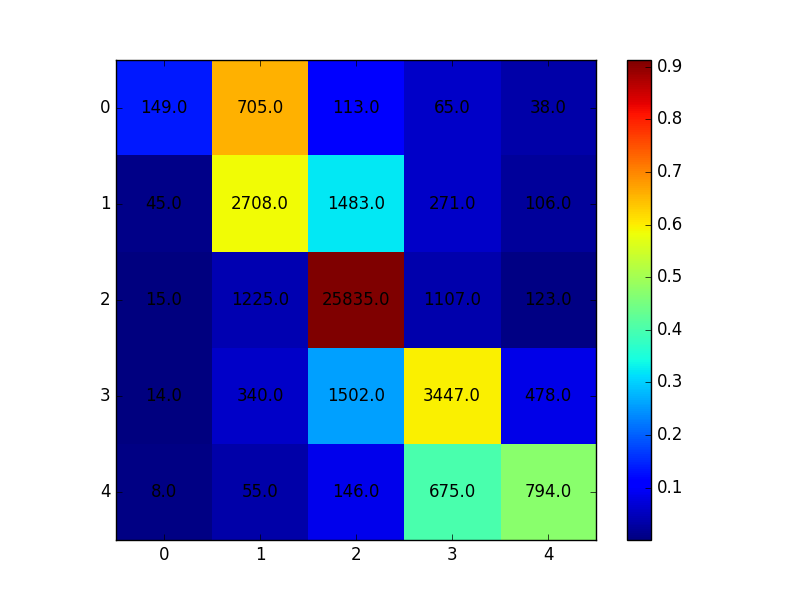
\includegraphics[width=0.7\linewidth]{ps3_1_c_c_dev}
\caption{Confusion Matrix on Dev Set}
\label{fig:ps3_1_c_c_dev}
\end{figure}
\subsubsection*{(d)}
\begin{figure}[H]
\centering
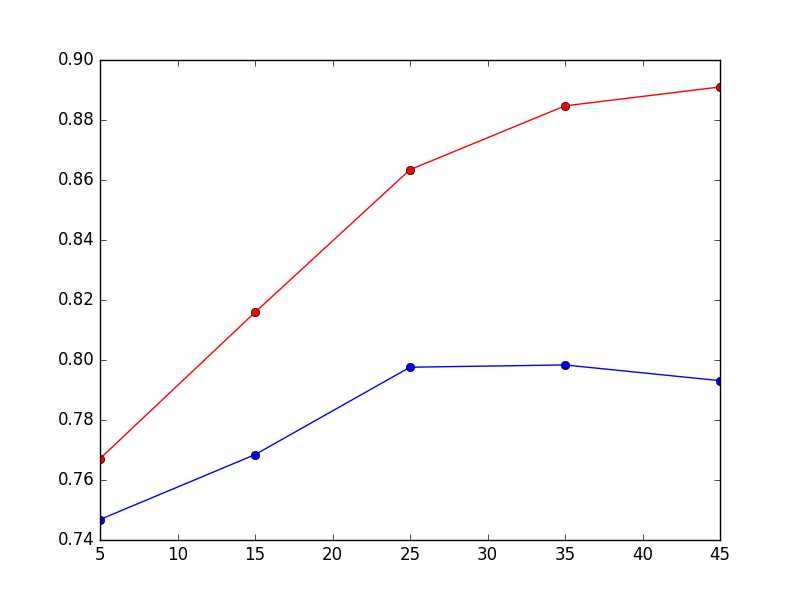
\includegraphics[width=0.7\linewidth]{ps3_1_c_d}
\caption{Accuracy on Training and Dev Set over wvecDims}
\label{fig:ps3_1_c_d}
\end{figure}
\newpage

\section{2-Layer Deep RNN's}
\subsection*{(a)}
\begin{align*}
\delta^{(s)} &= \hat{y} - y \\
\nabla_U J &= \delta^{(s)} (h^{(2)})^T \\
\nabla_{b^{(s)}} J &= \delta^{(s)} \\
\\
\delta^{(2)} &= f'(h^{(2)}) \circ (U^T \delta^{(s)}) \\
\nabla_{W^{(2)}} J &= \delta^{(2)} (h^{(1)})^T \\
\nabla_{b^{(2)}} J &= \delta^{(2)} \\
\\
\delta^{(1)} &= f'(h^{(1)}) \circ (({W^{(2)}})^T \delta^{(2)} + \delta_{above}) \\
\nabla_{W^{(1)}} J &= \delta^{(1)} \left[h^{(1)}_{left}; h^{(1)}_{right} \right]^T \\
\nabla_{b^{(1)}} J &= \delta^{(1)} \\
\\
\delta_{below} &= (W^{(1)})^T \delta^{(1)} \\
\nabla_{[L_{left}; L_{right}]} J &= \delta_{below}
\end{align*}
\subsection*{(b)}
Please see code files for details.
\subsection*{(c)}
\subsubsection*{(a)}
\begin{figure}[H]
\centering
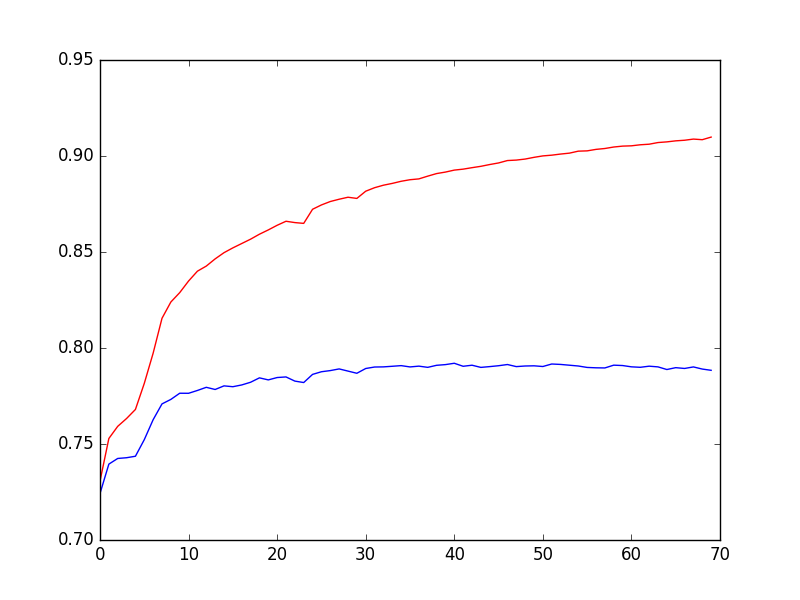
\includegraphics[width=0.7\linewidth]{ps3_2_c_a}
\caption{}
\label{fig:ps3_2_c_a}
\end{figure}
\subsubsection*{(b)}
\begin{figure}[H]
\centering
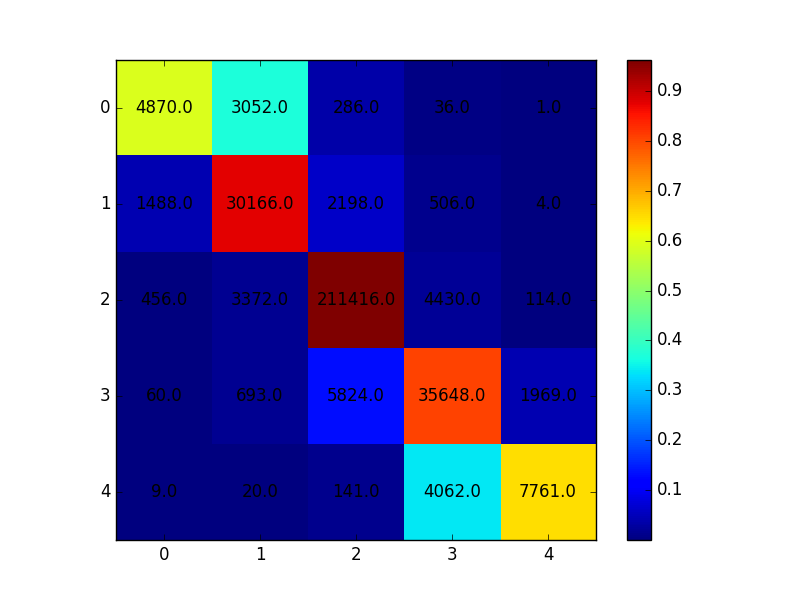
\includegraphics[width=0.7\linewidth]{ps3_2_c_b_train}
\caption{Confusion Matrix on Training Set}
\label{fig:ps3_2_c_b_train}
\end{figure}
\begin{figure}[H]
\centering
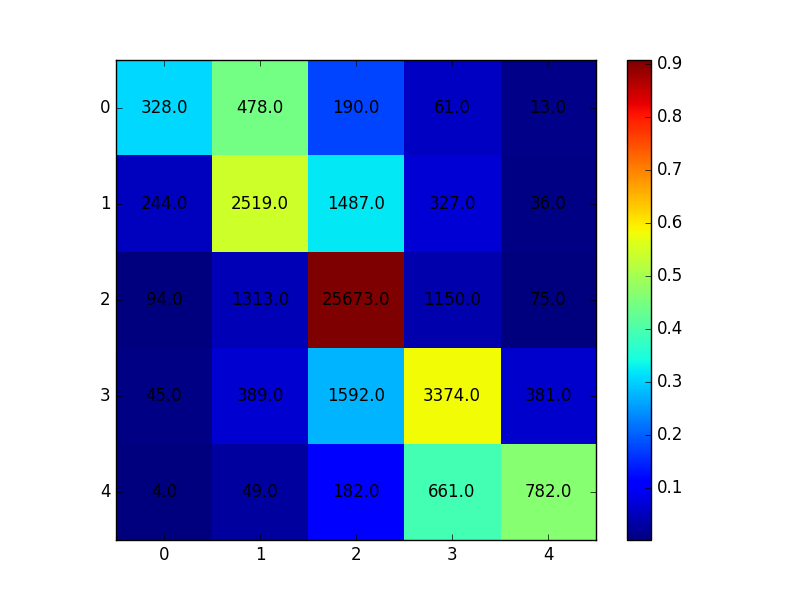
\includegraphics[width=0.7\linewidth]{ps3_2_c_b_dev}
\caption{Confusion Matrix on Dev Set}
\label{fig:ps3_2_c_b_dev}
\end{figure}

\subsubsection*{(c)}
Model RNN2 performs better on training set while worse on dev set, which indicates a typical problem of over fitting.
\subsubsection*{(d)}
\begin{figure}[H]
\centering
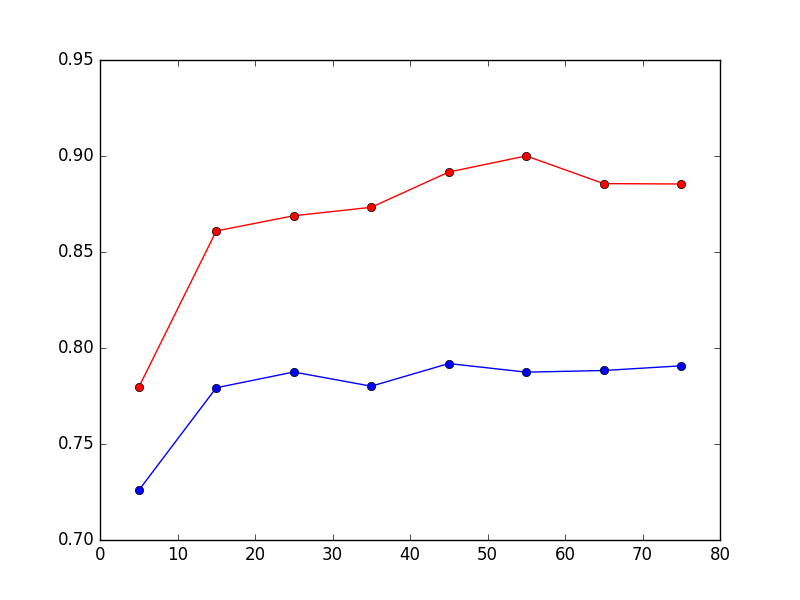
\includegraphics[width=0.7\linewidth]{ps3_2_c_d}
\caption{Accuracy on Training and Dev Set over middleDims}
\label{fig:ps3_2_c_d}
\end{figure}
\subsection*{(d)}
To be updated.
\subsection*{(e)}
To be updated.
\subsection*{(f)}
To be updated.
\section{Extra Credit: Recursive Neural Tensor Networks}
To be updated.
\end{document}